%!TEX root = main.tex


\chapter{Technical Prerequisites}\label{ch:tech_prereq}

Our approach to causal inference is (like most other approaches) based on probability theory. Many results and conventions will be familiar to readers, and these are collected in Section \ref{sec:standard_prob}.

Less likely to be familiar to readers is the string diagram notation we use to represent probabilistic functions. This is a notation created for reasoning about abstract Markov categories, and is somewhat different to existing graphical languages. The main difference is that in our notation wires represent variables and boxes (which are like nodes in directed acyclic graphs) represent probabilistic functions. Standard directed acyclic graphs annotate nodes with variable names and represent probabilistic functions implicitly. The advantage of explicitly representing probabilistic functions is that we can write equations involving graphics. It is introduced in Section \ref{ssec:mken_diagrams}.

We also extend the theory of probability to a theory of probability sets, which we introduce in Section \ref{sec:probability_sets}. This section goes over some ground already trodden by Section \ref{sec:standard_prob}; this structure was chosen so that people familiar with the Section \ref{sec:standard_prob} can skip to Section \ref{sec:probability_sets} for relevant generalisations to probability sets. Two key ideas introduced here are \emph{uniform conditional probability}, similar but not identical to conditional probability, and \emph{extended conditional independence} as introduced by \citet{constantinou_extended_2017}, similar but not identical to regular conditional independence.

We finally introduce the assumption of \emph{validity}, which ensures that probability sets constructed by ``assembling'' collections of uniform conditionals are non-empty.

This is a reference chapter -- a reader who is already quite familiar with probability theory may skip to Chapter \ref{ch:2p_statmodels}. Where necessary, references back to theorems and definitions in this chapter are given. In Chapter \ref{ch:evaluating_decisions}, we will introduce one additional probabilistic primitive: \emph{combs}, as we feel that additional context is helpful for understanding them.

\section{Conventions}

One of the unusual conventions in this thesis is the notation of uniform conditional probability. Given a set of probability distributions $\prob{P}_C:=\{\prob{P}_\alpha|\alpha\in C\}$ on a common sample space $(\Omega,\sigalg{F})$ with variables $\RV{X}:\Omega\to X$ and $\RV{Y}:\Omega\to Y$, $\prob{P}^{\RV{Y}|\RV{X}}_C$ represents a Markov kernel $X\kto Y$ that satisfies the definition of the distribution of $\RV{Y}$ given $\RV{X}$ (Definition \ref{def:disint}) for every $\alpha\in C$, while $\prob{P}_\alpha^{\RV{Y}|\RV{X}}$ is a conditional distribution only for $\alpha$. There are two unusual feature: firstly, it is more common to write a conditional distribution $\prob{P}(\RV{Y}|\RV{X})$ and secondly, the subscript indicating the ``domain of validity'' of the conditional probability is unusual.

Because this thesis uses sets of probability measures rather than single probability measures, in general a conditional distribution may be valid only for some subset of the probability measures, and always including a subscript indicating which subset or element for which a conditional distribution is valid avoids any ambiguity about this. Avoiding notation of the form $\prob{P}(\RV{Y}|\RV{X})$ is an aesthetic preference; writing a conditional distribution like this suggests $\prob{P}(\RV{Y}|\RV{X})$ is the result of function composition between $\prob{P}$ and some function denoted ``$\RV{Y}|\RV{X}$''. However, conditional probabilities are not given by composition of functions like this.

\begin{center}
\begin{tabular}{ |c|c|c| } 
 \hline
 Name & notation & meaning \\
 \hline
 Iverson bracket & $\llbracket \cdot \rrbracket$ & Function equal to 1 if $\cdot$ is true, false otherwise \\ 
 Identity function & $\mathrm{idf}_X$ & Identity function $X\to X$\\
 Identity kernel & $\mathrm{id}_{X}$ & Kernel associated with the identity function $X\to X$\\
 \hline
\end{tabular}
\end{center}

\section{Probability Theory}

\subsection{Standard Probability Theory}\label{sec:standard_prob}

\subsubsection{$\sigma$-algebras}

\begin{definition}[Sigma algebra]
Given a set $A$, a $\sigma$-algebra $\mathcal{A}$ is a collection of subsets of $A$ where
\begin{itemize}
	\item $A\in \mathcal{A}$ and $\emptyset\in \mathcal{A}$
	\item $B\in \mathcal{A}\implies B^C\in\mathcal{A}$
	\item $\mathcal{A}$ is closed under countable unions: For any countable collection $\{B_i|i\in Z\subset \mathbb{N}\}$ of elements of $\mathcal{A}$, $\cup_{i\in Z}B_i\in \mathcal{A}$ 
\end{itemize}
\end{definition}

\begin{definition}[Measurable space]
A measurable space $(A,\mathcal{A})$ is a set $A$ along with a $\sigma$-algebra $\mathcal{A}$.
\end{definition}

\begin{definition}[Sigma algebra generated by a set]
Given a set $A$ and an arbitrary collection of subsets $U\supset\mathscr{P}(A)$, the $\sigma$-algebra generated by $U$, $\sigma(U)$, is the smallest $\sigma$-algebra containing $U$.
\end{definition}

\paragraph{Common $\sigma$ algebras}

For any $A$, $\{\emptyset,A\}$ is a $\sigma$-algebra. In particular, it is the only sigma algebra for any one element set $\{*\}$.

For countable $A$, the power set $\mathscr{P}(A)$ is known as the discrete $\sigma$-algebra.

Given $A$ and a collection of subsets of $B\subset\mathscr{P}(A)$, $\sigma(B)$ is the smallest $\sigma$-algebra containing all the elements of $B$. 

If $A$ is a topological space with open sets $T$, $\mathcal{B}(\mathbb{R}):=\sigma(T)$ is the \emph{Borel $\sigma$-algebra} on $A$.

If $A$ is a separable, completely metrizable topological space, then $(A,\mathcal{B}(A))$ is a \emph{standard measurable set}. All standard measurable sets are isomorphic to either $(\mathbb{R},B(\mathbb{R}))$ or $(C,\mathscr{P}(C))$ for denumerable $C$ \citep[Chap. 1]{cinlar_probability_2011}.

\subsubsection{Probability measures and Markov kernels}

\begin{definition}[Probability measure]
Given a measurable space $(E,\sigalg{E})$, a map $\mu:\sigalg{E}\to [0,1]$ is a \emph{probability measure} if
\begin{itemize}
	\item $\mu(E)=1$, $\mu(\emptyset)=0$
	\item Given countable collection $\{A_i\}\subset\mathscr{E}$, $\mu(\cup_{i} A_i) = \sum_i \mu(A_i)$
\end{itemize}
\end{definition}

\begin{notation}[Set of all probability measures]
The set of all probability measures on $(E,\sigalg{E})$ is written $\Delta(E)$.
\end{notation}

\begin{definition}[Markov kernel]
Given measurable spaces $(E,\sigalg{E})$ and $(F,\sigalg{F})$, a \emph{Markov kernel} or \emph{stochastic function} is a map $\kernel{M}:E\times\sigalg{F}\to [0,1]$ such that
\begin{itemize}
	\item The map $\kernel{M}(A|\cdot):x\mapsto \kernel{M}(A|x)$ is $\sigalg{E}$-measurable for all $A\in \sigalg{F}$
	\item The map $\kernel{M}(\cdot|x):A\mapsto \kernel{M}(A|x)$ is a probability measure on $(F,\sigalg{F})$ for all $x\in E$
\end{itemize}
\end{definition}

\begin{notation}[Signature of a Markov kernel]
Given measurable spaces $(E,\sigalg{E})$ and $(F,\sigalg{F})$ and $\kernel{M}:E\times\sigalg{F}\to [0,1]$, we write the signature of $\kernel{M}:E\kto F$, read ``$\kernel{M}$ maps from $E$ to probability measures on $F$''.
\end{notation}

\begin{definition}[Deterministic Markov kernel]
A \emph{deterministic} Markov kernel $\kernel{A}:E\to \Delta(\mathcal{F})$ is a kernel such that $\kernel{A}_x(B)\in\{0,1\}$ for all $x\in E$, $B\in\mathcal{F}$.
\end{definition}

\paragraph{Common probability measures and Markov kernels}

\begin{definition}[Dirac measure]
The \emph{Dirac measure} $\delta_x\in \Delta(X)$ is a probability measure such that $\delta_x(A)=\llbracket x\in A \rrbracket$
\end{definition}

\begin{definition}[Markov kernel associated with a function]
Given measurable $f:(X,\sigalg{X})\to (Y,\sigalg{Y})$, $\kernel{F}_f:X\kto Y$ is the Markov kernel given by $x\mapsto \delta_{f(x)}$
\end{definition}

\begin{definition}[Markov kernel associated with a probability measure]
Given $(X,\sigalg{X})$, a one-element measurable space $(\{*\},\{\{*\},\emptyset\})$ and a probability measure $\mu\in \Delta(X)$, the associated Markov kernel $\kernel{Q}_\mu:\{*\}\kto X$ is the unique Markov kernel $*\mapsto \mu$
\end{definition}

\begin{lemma}[Products of functional kernels yield function composition]\label{lem:func_kern_product}
Given measurable $f:X\to Y$ and $g:Y\to Z$, $\kernel{F}_f\kernel{F}_g = \kernel{F}_{g\circ f}$.
\end{lemma}

\begin{proof}
\begin{align}
    (\kernel{F}_{f}\kernel{F}_g)_x(A) &= \int_X (\kernel{F}_g)_y(A) d(\kernel{F}_f)_x(y)\\
                                      &= \int_X \delta_{g(y)}(A) d\delta_{f(x)}(y)\\
                                      &= \delta_{g(f(x))} (A)\\
                                      &= (\kernel{F}_{g\circ f})_x(A) 
\end{align}
\end{proof}

\subsubsection{Variables, conditionals and marginals}

\begin{definition}[Variable]\label{def:variable}
Given a measurable space $(\Omega,\sigalg{F})$ and a measurable space of values $(X,\sigalg{X})$, an \emph{$X$-valued variable} is a measurable function $\RV{X}:(\Omega,\sigalg{F})\to (X,\sigalg{X})$.
\end{definition}

\begin{definition}[Sequence of variables]
Given a measurable space $(\Omega,\sigalg{F})$ and two variables $\RV{X}:(\Omega,\sigalg{F})\to (X,\sigalg{X})$, $\RV{Y}:(\Omega,\sigalg{F})\to (Y,\sigalg{Y})$, $(\RV{X},\RV{Y}):\Omega\to X\times Y$ is the variable $\omega\mapsto (\RV{X}(\omega),\RV{Y}(\omega))$.
\end{definition}

\begin{definition}[Marginal distribution]\label{def:pushforward}
Given a probability space $(\mu,\Omega,\sigalg{F})$ and a variable $\RV{X}:\Omega\to (X,\sigalg{X})$, the \emph{marginal distribution} of $\RV{X}$ with respect to $\mu$, $\mu^{\RV{X}}:\sigalg{X}\to [0,1]$ by $\mu^{\RV{X}}(A):=\mu(\RV{X}^{-1}(A))$ for any $A\in \sigalg{X}$.
\end{definition}

\begin{definition}[Conditional distribution]\label{def:disint}
Given a probability space $(\mu,\Omega,\sigalg{F})$ and variables $\RV{X}:\Omega\to X$, $\RV{Y}:\Omega\to Y$, the \emph{conditional distribution} of $\RV{Y}$ given $\RV{X}$ is any Markov kernel $\mu^{\RV{Y}|\RV{X}}:X\kto Y$ such that
\begin{align}
	\mu^{\RV{XY}}(A\times B)&=\int_{A} \mu^{\RV{Y}|\RV{X}}(B|x) \mathrm{d}\mu^{\RV{X}}(x) &\forall A\in \sigalg{X}, B\in \sigalg{Y}\\
	&\iff\\
	\mu^{\RV{XY}}&= \tikzfig{disint_def}\label{eq:conditional} 
\end{align}
\end{definition}

\subsubsection{Markov kernel product notation}\label{ssec:product_notation}

Three pairwise \emph{product} operations involving Markov kernels can be defined: measure-kernel products, kernel-kernel products and kernel-function products. These are analagous to row vector-matrix products, matrix-matrix products and matrix-column vector products respectively.

 , $\RV{T}:Y\to T$, $\kernel{M}:X\to \Delta(\sigalg{Y})$ and $\kernel{N}:Y\to \Delta(\sigalg{Z})$

\begin{definition}[Measure-kernel product]
Given $\mu\in \Delta(\mathcal{X})$ and $\kernel{M}:X\kto Y$, the \emph{measure-kernel product} $\mu\kernel{M}\in \Delta(Y)$ is given by
\begin{align}
\mu\kernel{M} (A) := \int_X \kernel{M}(A|x) \mu(\mathrm{d}x)
\end{align}
for all $A\in \sigalg{Y}$.
\end{definition}

\begin{definition}[Kernel-kernel product]
Given $\kernel{M}:X\kto Y$ and $\kernel{N}:Y\kto Z$, the \emph{kernel-kernel product} $\kernel{M}\kernel{N}:X\kto Z$ is given by
\begin{align}
\kernel{MN} (A|x) := \int_Y \kernel{N}(A|x) \kernel{M}(\mathrm{d}y|x)
\end{align}
for all $A\in \sigalg{Z}$, $x\in X$.
\end{definition}

\begin{definition}[Kernel-function product]
Given $\kernel{M}:X\kto Y$ and $f:Y\to Z$, the \emph{kernel-function product} $\kernel{M}f:X\to Z$ is given by
\begin{align}
\kernel{M}f (x) := \int_Y f(y)\kernel{N}(\mathrm{d}y|x)
\end{align}
for all $x\in X$.
\end{definition}

\begin{definition}[Tensor product]
Given $\kernel{M}:X\kto Y$ and $\kernel{L}:W\kto Z$, the tensor product $\kernel{M}\otimes\kernel{N}:X\times W\kto Y\times Z$ is given by
\begin{align}
	(\kernel{M}\otimes\kernel{L})(A\times B|x,w):=\kernel{M}(A|x)\kernel{L}(B|w)
\end{align}
For all $x\in X$, $w\in W$, $A\in \sigalg{Y}$ and $B\in \sigalg{Z}$.
\end{definition}

All products are associative \citep[Chapter 1]{cinlar_probability_2011}.

One application of the product notation is that marginal distributions can be alternatively defined in terms of a kernel product, as shown in Lemma \ref{lem:pushf_kprod}.

\begin{lemma}[Marginal distribution as a kernel product]\label{lem:pushf_kprod}
Given a probability space $(\mu,\Omega,\sigalg{F})$ and a variable $\RV{X}:\Omega\to (X,\sigalg{X})$, define $\kernel{F}_{\RV{X}}:\Omega\kto X$ by $\kernel{F}_{\RV{X}}(A|\omega)=\delta_{\RV{X}(\omega)}(A)$, then
\begin{align}
	\mu^{\RV{X}} = \mu\kernel{F}_{\RV{X}}
\end{align}
\end{lemma}

\begin{proof}
Consider any $A\in \sigalg{X}$.
\begin{align}
	\mu \kernel{F}_{\RV{X}}(A) &= \int_\Omega \delta_{\RV{X}(\omega)}(A) \mathrm{d}\mu(\omega)\\
	&= \int_{\RV{X}^{-1}(\omega)} \mathrm{d}\mu(\omega)\\
	&= \mu^{\RV{X}}(A)
\end{align}
\end{proof}

\subsubsection{Semidirect product}

Given a marginal $\mu^{\RV{X}}$ and a conditional $\mu^{\RV{Y}|\RV{X}}$, the product of the two yields the marginal distribution of $\RV{Y}$: $\mu^{\RV{Y}}=\mu^{\RV{X}}\mu^{\RV{Y}|\RV{X}}$. We define another product -- the \emph{semidirect} product $\odot$ -- as the product that yields the joint distribution of $(\RV{X},\RV{Y})$: $\mu^{\RV{XY}}=\mu^{\RV{X}}\odot\mu^{\RV{Y}|\RV{X}}$. The semidirect product is associative (Lemma \ref{lem:sdp_assoc})

\begin{definition}[Semidirect product]\label{def:copyproduct}
Given $\prob{K}:X\kto Y$ and $\prob{L}:Y\times X\kto Z$, the semidirect product $\prob{K}\cprod\prob{L}:X\to Y\times Z$ is given by
\begin{align}
    (\prob{K}\cprod\prob{L})(A\times B|x) &= \int_A \prob{L}(B|y,x)\prob{K}(dy|x)&\forall A\in \sigalg{Y},B\in\sigalg{Z}
\end{align}
\end{definition}


\begin{lemma}[Semidirect product is associative]\label{lem:sdp_assoc}
Given $\prob{K}:X\kto Y$, $\prob{L}:Y\times X\kto Z$ and $\prob{M}:Z\times Y\times X\kto W$
\begin{align}
    (\prob{K}\odot \prob{L})\odot \prob{Z} &= \prob{K}\odot(\prob{L}\odot\prob{Z})\\
\end{align}
\end{lemma}

\begin{proof}
\begin{align}
    (\prob{K}\odot \prob{L})\odot \prob{M} &= \tikzfig{odot_assoc_1}\\
                                            &=  \tikzfig{odot_assoc_2}\\
                                            &= \prob{K}\odot (\prob{L}\odot \prob{M})
\end{align}
\end{proof}

The semidirect product can be used to define a notion of almost sure equality: two kernels $\kernel{K}:X\kto Y$ and $\kernel{L}:X\kto Y$ are $\mu$-almost surely equal if $\mu\odot \kernel{K}=\mu\odot \kernel{L}$. This is identical to the notion of almost sure equality in \citet{cho_disintegration_2019}, who shows that under the assumption that $(Y,\sigalg{Y})$ is countably generated, $\kernel{K}\overset{\mu}{\cong}\kernel{L}$ if and only if $\kernel{K}=\kernel{L}$ $\mu$-almost everywhere.

\begin{definition}[Almost sure equality]\label{def:asequal_pspace}
Two Markov kernels $\kernel{K}:X\kto Y$ and $\kernel{L}:X\kto Y$ are almost surely equal $\overset{\prob{P}_C}{\cong}$ with respect to a probability space $(\mu,X,\sigalg{X})$, written $\kernel{K}\overset{\mu}{\cong}\kernel{L}$ if
\begin{align}
    \mu\odot \kernel{K}=\mu\odot \kernel{L}
\end{align}
\end{definition}

\begin{theorem}
Given $(\mu,X,\sigalg{X})$, $\kernel{K}:X\kto Y$ and $\kernel{L}:X\kto Y$, $\kernel{K}\overset{\mu}{\cong}\kernel{L}$ if and only if, defining $U:=\{x|\exists A\in\sigalg{Y}: \kernel{K}(A|x)\neq\kernel{L}(A|x)\}$, $\mu(U)=0$.
\end{theorem}

\begin{proof}
\citet{cho_disintegration_2019} proposition 5.4.
\end{proof}

We often want to talk about almost sure equality of two different versions $\kernel{K}$ and $\kernel{L}$ of a conditional distribution $\prob{P}^{\RV{Y}|\RV{X}}$ with respect to some ambient probability space $(\prob{P},\Omega,\sigalg{F})$. This simply means $\kernel{K}$ and $\kernel{L}$ satisfy Definition \ref{def:disint} with respect to $\prob{P}$, $\RV{X}$ and $\RV{Y}$, and they are almost surely equal with respect to the marginal $\prob{P}^{\RV{X}}$. Tthe relevant variables are usually obvious from the context and we leave them implicit and we will write $\kernel{K}\overset{\prob{P}}{\cong}\kernel{L}$. If the relevant marginal is ambiguous, we will instead write $\kernel{K}\overset{\prob{P}^{\RV{X}}}{\cong}\kernel{L}$

\begin{definition}[Almost sure equality with respect to a pair of variables]
Given $(\prob{P},\Omega,\sigalg{F})$ and $\RV{X}:\Omega\to X$, $\RV{Y}:\Omega\to Y$, two Markov kernels $\kernel{K}:X\kto Y$ and $\kernel{L}:X\kto Y$ are $\RV{X}$-almost surely equal with respect to $\prob{P}$, written $\kernel{K}\overset{\prob{P}}{\cong}\kernel{L}$, if they are almost surely equal with respect to the marginal $\prob{P}^{\RV{X}}$.
\end{definition}



\section{String Diagrams}\label{ssec:mken_diagrams}

We make use of string diagram notation for probabilistic reasoning. Graphical models are often employed in causal reasoning, and string diagrams are a kind of graphical notation for representing Markov kernels. The notation comes from the study of Markov categories, which are abstract categories that represent models of the flow of information. For our purposes, we don't use abstract Markov categories but instead focus on the concrete category of Markov kernels on standard measurable sets.

A coherence theorem exists for string diagrams and Markov categories. Applying planar deformation or any of the commutative comonoid axioms to a string diagram yields an equivalent string diagram. The coherence theorem establishes that any proof constructed using string diagrams in this manner corresponds to a proof in any Markov category \citep{selinger_survey_2011}. More comprehensive introductions to Markov categories can be found in \citet{fritz_synthetic_2020,cho_disintegration_2019}.

\subsection{Elements of string diagrams}\label{sec:string_diagram_elements}

In the string, Markov kernels are drawn as boxes with input and output wires, and probability measures (which are Markov kernels with the domain $\{*\}$) are represented by triangles:

\begin{align}
\kernel{K}&:=\begin{tikzpicture}[baseline={([yshift=-.5ex]current bounding box.center)}]
    \path (0,0) node (A) {}
    ++ (0.5,0) node[kernel] (K) {$\kernel{K}$}
    ++ (0.5,0) node (B) {};
    \draw (A) -- (K) -- (B);
\end{tikzpicture}\\
\mu&:= \begin{tikzpicture}[baseline={([yshift=-.5ex]current bounding box.center)}]
    \path (0,0) node[dist] (K) {$\kernel{P}$}
    ++ (0.5,0) node (B) {};
    \draw (K) -- (B);
\end{tikzpicture}
\end{align}

Given two Markov kernels $\kernel{L}:X\kto Y$ and $\kernel{M}:Y\kto Z$, the product $\kernel{L}\kernel{M}$ is represented by drawing them side by side and joining their wires:

\begin{align}
    \kernel{L}\kernel{M}:= \begin{tikzpicture}[baseline={([yshift=-.5ex]current bounding box.center)}]
    \path (0,0) node (A) {$X$}
    ++ (0.5,0) node[kernel] (K) {$\kernel{K}$}
    ++ (0.7,0) node[kernel] (M) {$\kernel{M}$}
    ++ (0.5,0) node (B) {$Z$};
    \draw (A) -- (K) -- (M) -- (B);
\end{tikzpicture}
\end{align}

Given kernels $\kernel{K}:W\kto Y$ and $\kernel{L}:X\kto Z$, the tensor product $\kernel{K}\otimes\kernel{L}:W\times X\kto Y\times Z$ is graphically represented by drawing kernels in parallel:

\begin{align}
    \kernel{K}\otimes \kernel{L}&:=\begin{tikzpicture}[baseline={([yshift=-.5ex]current bounding box.center)}]
    \path (0,0) node (A) {$W$}
    ++ (0.5,0) node[kernel] (K) {$\kernel{K}$}
    ++ (0.5,0) node (B) {$Y$};
    \path (0,-0.5) node (C) {$X$}
    ++ (0.5,0) node[kernel] (L) {$\kernel{L}$}
    ++ (0.5,0) node (D) {$Z$};
    \draw (A) -- (K) -- (B);
    \draw (C) -- (L) -- (D);
\end{tikzpicture}
\end{align}

Given $\prob{K}:X\kto Y$ and $\prob{L}:Y\times X\kto Z$, the semidirect product is graphically represented by connecting $\kernel{K}$ and $\kernel{L}$ and keeping an extra copy

\begin{align}
    \prob{K}\cprod\prob{L}:&= \text{copy}_X(\prob{K}\otimes \text{id}_X)(\text{copy}_Y\otimes\text{id}_X )(\text{id}_Y \otimes \prob{L})\\
                            &= \tikzfig{copy_product}
\end{align}

A space $X$ is identified with the identity kernel $\mathrm{id}^X:X\to \Delta(\sigalg{X})$. A bare wire represents the identity kernel:

\begin{align}
\mathrm{Id}^X:=\begin{tikzpicture}
\path (0,0) node (X) {$X$}
++(2,0) node (Y) {$X$};
\draw (X) -- (Y);
\end{tikzpicture}
\end{align}

Product spaces $X\times Y$ are identified with tensor product of identity kernels $\mathrm{id}^X\otimes \mathrm{id}^Y$. These can be represented either by two parallel wires or by a single wire representing the identity on the product space $X\times Y$:
\begin{align}
X\times Y \cong \mathrm{Id}^X\otimes \mathrm{Id}^Y &:= 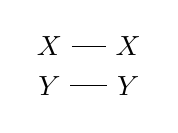
\begin{tikzpicture}
\path (0,0) node (E) {$X$}
++(1,0) node (F) {$X$}
(0,-0.5) node (F1) {$Y$}
+(1,0) node (G) {$Y$};
\draw (E) -- (F);
\draw (F1) -- (G);
\end{tikzpicture}\\
&= 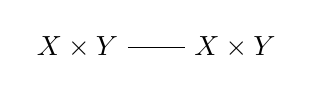
\begin{tikzpicture}
\path (0,0) node (X) {$X\times Y$}
++(2,0) node (Y) {$X\times Y$};
\draw (X) -- (Y);
\end{tikzpicture}
\end{align}

A kernel $\kernel{L}:X\to \Delta(\mathcal{Y}\otimes\mathcal{Z})$ can be written using either two parallel output wires or a single output wire, appropriately labeled:

\begin{align}
&\begin{tikzpicture}
\path (0,0) node (E) {$X$}
++ (1,0) node[kernel] (L) {$\kernel{L}$}
++ (1,0.15) node (F) {$Y$}
+(0,-0.3) node (G) {$Z$};
\draw (E) -- (L);
\draw ($(L.east) + (0,0.15)$) -- (F);
\draw ($(L.east)+ (0,-0.15)$) -- (G);
\end{tikzpicture}\\
&\equiv\\
&\begin{tikzpicture}
\path (0,0) node (E) {$X$}
++ (1,0) node[kernel] (L) {$\kernel{L}$}
++ (1.5,0) node (F) {$Y\times Z$};
\draw (E) -- (L) -- (F);
\end{tikzpicture}
\end{align}

We read diagrams from left to right (this is somewhat different to \citet{fritz_synthetic_2020,cho_disintegration_2019,fong_causal_2013} but in line with \citet{selinger_survey_2011}), and any diagram describes a set of nested products and tensor products of Markov kernels. There are a collection of special Markov kernels for which we can replace the generic ``box'' of a Markov kernel with a diagrammatic elements that are visually suggestive of what these kernels accomplish.

\subsection{Special maps}

\begin{definition}[Identity map]
The identity map $\text{id}_X:X\kto X$ defined by $(\text{id}_X)(A|x)= \delta_x(A)$ for all $x\in X$, $A\in\sigalg{X}$, is represented by a bare line.
\begin{align}
    \mathrm{id}_X&:=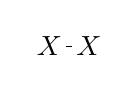
\begin{tikzpicture}[baseline={([yshift=-.5ex]current bounding box.center)}]
    \path (0,0) node (A) {$X$} ++ (0.5,0) node (B) {$X$};
    \draw (A) -- (B);
\end{tikzpicture}
\end{align}
\end{definition}

\begin{definition}[Erase map]
Given some 1-element set $\{*\}$, the erase map $\text{del}_X:X\kto \{*\}$ is defined by $(\text{del}_X)(*|x) = 1$ for all $x\in X$. It ``discards the input''. It looks like a lit fuse:
\begin{align}
    \text{del}_X&:=\begin{tikzpicture}[baseline={([yshift=-.5ex]current bounding box.center)}]
    \path (0,0) ++ (1,0) node (B) {$X$};
    \draw[-{Rays[n=8]}] (A) -- (B);
\end{tikzpicture}
\end{align}
\end{definition}

\begin{definition}[Swap map]
The swap map $\text{swap}_{X,Y}:X\times Y\kto Y\times X$ is defined by $(\text{swap}_{X,Y})(A\times B|x,y)=\delta_x(B)\delta_y(A)$ for $(x,y)\in X\times Y$, $A\in \sigalg{X}$ and $B\in \sigalg{Y}$. It swaps two inputs and is represented by crossing wires:
\begin{align}
    \text{swap}_{X,Y} &:=  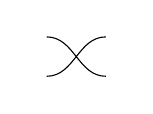
\begin{tikzpicture}[baseline={([yshift=-.5ex]current bounding box.center)}]
        \path (0,0) node (A) {} 
        + (0,-0.5) node (B) {}
        ++ (1,0) node (C) {}
        + (0,-0.5) node (D) {};
        \draw (A) to [out=0,in=180] (D) (B) to [out=0, in=180] (C);
    \end{tikzpicture}
\end{align}
\end{definition}

\begin{definition}[Copy map]
The copy map $\text{copy}_X:X\kto X\times X$ is defined by $(\text{copy}_X)(A\times B|x)=\delta_x(A)\delta_x(B)$ for all $x\in X$, $A,B\in \sigalg{X}$. It makes two identical copies of the input, and is drawn as a fork:
\begin{align}
    \text{copy}_X&:=\begin{tikzpicture}[baseline={([yshift=-.5ex]current bounding box.center)}]
    \path (0,0) node (A) {$X$} 
    ++ (0.5,0) node[copymap] (copy0) {}
    ++ (0.5,0.15) node (B) {$X$}
    + (0,-0.3) node (C) {$X$};
    \draw (A) -- (copy0) to [out=45,in=180] (B) (copy0) to [out=-45, in=180] (C);
\end{tikzpicture}
\end{align}
\end{definition}

\begin{definition}[$n$-fold copy map]
The $n$-fold copy map $\text{copy}^n_X:X\kto X^n$ is given by the recursive definition
\begin{align}
    \text{copy}^1_X &= \text{copy}_X\\
    \text{copy}^n_X &= \tikzfig{n_fold_copy} &n>1
\end{align}
\end{definition}

\paragraph{Plates}

In a string diagram, a plate that is annotated $i\in A$ means the tensor product of the $|A|$ elements that appear inside the plate. A wire crossing from outside a plate boundary to the inside of a plate indicates an $|A|$-fold copy map, which we indicate by placing a dot on the plate boundary. For our purposes, we do not define anything that allows wires to cross from the inside of a plate to the outside; wires must terminate within the plate.

Thus, given $\kernel{K}_i:X\kto Y$ for $i\in A$,

\begin{align}
    \bigotimes_{i\in A} \kernel{K}_i &:= \tikzfig{plate_without_copymap}
    \text{copy}^{|A|}_X(\bigotimes_{i\in A} \kernel{K}_i) &:= \tikzfig{plate_with_copymap}
\end{align}

\subsection{Commutative comonoid axioms}

Diagrams in Markov categories satisfy the commutative comonoid axioms.

\begin{align}
    \tikzfig{ccom_lhs} = \tikzfig{ccom_rhs}\label{eq:ccom_1}
\end{align}
\begin{align}
    \tikzfig{ccom2_lhs} = \tikzfig{ccom2_mhs} = \tikzfig{ccom2_rhs}\label{eq:ccom2_del}
\end{align}
\begin{align}
    \tikzfig{ccom3_lhs} = \tikzfig{ccom3_rhs} \label{eq:ccom3_swap}
\end{align}
as well as compatibility with the monoidal structure
\begin{align}
    \tikzfig{mstruct1_lhs} &= \tikzfig{mstruct1_rhs}\\
    \tikzfig{mstruct2_lhs} &= \tikzfig{mstruct2_rhs}
\end{align}
and the naturality of \emph{del}, which means that
\begin{align}
    \tikzfig{naturality_lhs} &= \tikzfig{naturality_rhs}\label{eq:nat}
\end{align}


\subsection{Manipulating String Diagrams}\label{sssec:string_diagram_manipulation}

Planar deformations along with the applications of Equations \ref{eq:ccom_1} through to Equation \ref{eq:nat} are almost the only rules we have for transforming one string diagram into an equivalent one. One further rule is given by Theorem \ref{th:fong_det_kerns}.

\begin{theorem}[Copy map commutes for deterministic kernels \citep{fong_causal_2013}]\label{th:fong_det_kerns}
For $\kernel{K}:X\kto Y$
\begin{align}
	\tikzfig{deterministic_copymap_commute}
\end{align}
holds iff $\kernel{K}$ is deterministic.
\end{theorem}

\subsubsection{Examples}

String diagrams can always be converted into definitions involving integrals and tensor products. A number of shortcuts can help to make the translations efficiently.

For arbitrary $\kernel{K}:X\times Y\kto Z$, $\kernel{L}:W\kto Y$

\begin{align}
    \tikzfig{identity_tensor_L} &= (\text{id}_X\otimes \kernel{L})\kernel{K}\\
    [(\text{id}_X\otimes \kernel{L})\kernel{K}](A|x,w) &= \int_{Y}\int_X   \kernel{K}(A|x',y')\kernel{L}(\mathrm{d}y'|w)\delta_x(\mathrm{d}x')\\
                                           &= \int_Y  \kernel{K}(A|x,y') \kernel{L}(dy'|w)
\end{align}

That is, an identity map ``passes its input directly to the next kernel''. 

For arbitrary $\kernel{K}: X\times Y\times Y\kto Z$:

\begin{align}
 \tikzfig{identity_tensor_copy} &= (\text{id}_X\otimes \text{copy}_Y)\kernel{K}\\
 [(\text{id}_X\otimes \text{copy}_Y)\kernel{K}](A|x,y) &= \int_Y\int_Y \kernel{K}(A|x,y',y'') \delta_y(\mathrm{d}y')\delta_y(\mathrm{d}y'')\\
                                           &= \kernel{K}(A|x,y,y)
\end{align}

That is, the copy map ``passes along two copies of its input'' to the next kernel in the product. 

For arbitrary $\kernel{K}:X\times Y\kto Z$

\begin{align}
    \tikzfig{swap_example} &= \text{swap}_{YX} \kernel{K}\\
    (\text{swap}_{YX}\kernel{K})(A|y,x) &= \int_{X\times Y} \kernel{K}(A|x',y')\delta_y(\mathrm{d}y')\delta_x(\mathrm{d}x')\\
                                        &= \kernel{K}(A|x,y)
\end{align}

The swap map before a kernel switches the input arguments.

For arbitrary $\kernel{K}:X\kto Y\times Z$

\begin{align}
    \tikzfig{swap_example_2} &= \kernel{K}\text{swap}_{YZ}\\
    (\kernel{K}\text{swap}_{YZ})(A\times B|x) &= \int_{Y\times Z} \delta_{y}(B)\delta_{z}(A)\kernel{K}(\mathrm{d}y\times\mathrm{d}z|x)\\
    &= \int_{B\times A} \kernel{K}(\mathrm{d}y\times\mathrm{d}z|x)\\
    &= \kernel{K}(B\times A|x)
\end{align}

Given $\kernel{K}:X\kto Y$ and $\kernel{L}:Y\kto Z$:

\begin{align}
	(\kernel{K}\cprod \kernel{L})(\mathrm{id}_{Y}\otimes \mathrm{del}_Z) &= \tikzfig{semidirect_K_L}\\
	 &= \tikzfig{semidirect_K_L_2} &\text{by Eq. \ref{eq:nat}}\\
	 &= \tikzfig{semidirect_K_L_3} &\text{by Eq. \ref{eq:ccom2_del}}
\end{align}

Thus the action of the $\text{del}$ map is to marginalise over the deleted wire. With integrals, we can write

\begin{align}
	(\kernel{K}\cprod \kernel{L})(\mathrm{id}_{Y}\otimes \mathrm{del}_Z)(A\times\{*\}|x) &= \int_{Y}\int_{\{*\}}\delta_y(A)\delta_{*}(\{*\})\kernel{L}(\mathrm{d}z|y)\kernel{K}(\mathrm{d}y|x)\\
	&= \int_A \kernel{K}(\mathrm{d}y|x)\\
	&= \kernel{K}(A|x)
\end{align}

\section{Probability Sets}\label{sec:probability_sets}


A probability set is a set of probability measures. This section establishes a number of useful properties of conditional probability with respect to probability sets. Unlike conditional probability with respect to a probability space, conditional probabilities don't always exist for probability sets. Where they do, however, they are almost surely unique and we can marginalise and disintegrate them to obtain other conditional probabilities with respect to the same probability set.

\begin{definition}[Probability set]
A probability set $\prob{P}_C$ on $(\Omega,\sigalg{F})$ is a collection of probability measures on $(\Omega,\sigalg{F})$. In other words it is a subset of $\mathscr{P}(\Delta(\Omega))$, where $\mathscr{P}$ indicates the power set.
\end{definition}

Given a probability set $\prob{P}_C$, we define marginal and conditional probabilities as probability measures and Markov kernels that satisfy Definitions \ref{def:pushforward} and \ref{def:disint} respectively for \emph{all} base measures in $\prob{P}_C$. There are generally multiple Markov kernels that satisfy the properties of a conditional probability with respect to a probability set, and this definition ensures that marginal and conditional probabilities are ``almost surely'' unique (Definition \ref{def:asequal}) with respect to probability sets.

\begin{definition}[Marginal probability with respect to a probability set]
Given a sample space $(\Omega,\sigalg{F})$, a variable $\RV{X}:\Omega\to X$ and a probability set $\prob{P}_C$, the marginal distribution $\prob{P}_C^{\RV{X}}=\prob{P}_\alpha^{\RV{X}}$ for any $\prob{P}_\alpha\in\prob{P}_C$ if a distribution satisfying this condition exists. Otherwise, it is undefined.
\end{definition}

\begin{definition}[Uniform conditional distribution]\label{def:cprob_pset}
Given a sample space $(\Omega,\sigalg{F})$, variables $\RV{X}:\Omega\to X$ and $\RV{Y}:\Omega\to Y$ and a probability set $\prob{P}_C$, a uniform conditional distribution $\prob{P}_C^{\RV{Y}|\RV{X}}$ is any Markov kernel $X\kto Y$ such that $\prob{P}_C^{\RV{Y}|\RV{X}}$ is an $\RV{Y}|\RV{X}$ conditional probability of $\prob{P}_\alpha$ for all $\prob{P}_\alpha\in \prob{P}_C$. If no such Markov kernel exists, $\prob{P}_C^{\RV{Y}|\RV{X}}$ is undefined.
\end{definition}

Given a conditional distribution $\mu^{\RV{ZY}|\RV{X}}$ we can define a higher order conditional $\mu^{\RV{Z}|(\RV{Y}|\RV{X})}$, which is a version of $\mu^{\RV{Z}|\RV{XY}}$. This is useful because uniform conditionals don't always exist, but we can use higher order conditionals to show that if a probability set $\prob{P}_C$ has a uniform conditional $\prob{P}_C^{\RV{ZY}|\RV{X}}$ then it also has a uniform conditional $\prob{P}_C^{\RV{Z}|\RV{XY}}$ (Theorems \ref{th:ho_cond_psets} and \ref{th:higher_order_conditionals}). Given $\mu^{\RV{XY}|\RV{Z}}$ and $\RV{X}:\Omega\to X$, $\RV{Y}:\Omega\to Y$ standard measurable, it has recently been proven that a higher order conditional $\mu^{\RV{Z}|(\RV{Y}|\RV{X})}$ exists \citet{bogachev_kantorovich_2020}, Theorem 3.5.

\begin{definition}[Higher order conditionals]
Given a probability space $(\mu,\Omega,\sigalg{F})$ and variables $\RV{X}:\Omega\to X$, $\RV{Y}:\Omega\to Y$ and $\RV{Z}:\Omega\to Z$, a higher order conditional $\mu^{\RV{Z}|(\RV{Y}|\RV{X})}:X\times Y\to Z$ is any Markov kernel such that, for some $\mu^{\RV{Y}|\RV{X}}$, 
\begin{align}
    \mu^{\RV{ZY}|\RV{X}}(B\times C|x) &=\int_B \mu^{\RV{Z}|(\RV{Y}|\RV{X})}(C|x,y)\mu^{\RV{Y}|\RV{X}}(dy|x)\\ 
    &\iff\\
    \mu^{\RV{ZY}|\RV{X}} &= \tikzfig{disintegration_existence}\label{eq:disint_def}
\end{align}
\end{definition}

\begin{definition}[Uniform higher order conditional]\label{def:ho_cprob_pset}
Given a sample space $(\Omega,\sigalg{F})$, variables $\RV{X}:\Omega\to X$, $\RV{Y}:\Omega\to Y$ and $\RV{Z}:\Omega\to Z$ and a probability set $\prob{P}_C$, if $\prob{P}_C^{\RV{ZY}|\RV{X}}$ exists then a uniform higher order conditional $\prob{P}_C^{\RV{Z}|(\RV{Y}|\RV{X})}$ is any Markov kernel $X\times Y\kto Z$ that is a higher order conditional of some version of $\prob{P}_C^{\RV{ZY}|\RV{X}}$. If no $\prob{P}_C^{\RV{ZY}|\RV{X}}$ exists, $\prob{P}_C^{\RV{Z}|(\RV{Y}|\RV{X})}$ is undefined.
\end{definition}

\begin{definition}[Almost sure equality]
Two Markov kernels $\kernel{K}:X\kto Y$ and $\kernel{L}:X\kto Y$ are $\prob{P}_C,\RV{X},\RV{Y}$-almost surely equal if for all $A\in\sigalg{X}$, $B\in \sigalg{Y}$, $\alpha\in C$
\begin{align}
    \int_A \kernel{K}(B|x)\prob{P}_\alpha^{\RV{X}}(\mathrm{d}x) = \int_A\kernel{L}(B|x)\prob{P}_\alpha^{\RV{X}}(\mathrm{d}x)
\end{align}
we write this as $\kernel{K}\overset{\prob{P}_C}{\cong}\kernel{L}$, as the variables $\RV{X}$ and $\RV{Y}$ are clear from the context.
\end{definition}

Equivalently, $\kernel{K}$ and $\kernel{L}$ are almost surely equal if the set $C:\{x|\exists B\in\sigalg{Y}:\kernel{K}(B|x)\neq\kernel{L}(B|x)\}$ has measure 0 with respect to $\prob{P}_\alpha^{\RV{X}}$ for all $\alpha\in C$.

\subsection{Almost sure equality}

Two Markov kernels are almost surely equal with respect to a probability set $\prob{P}_C$ if the semidirect product $\odot$ of all marginal probabilities of $\prob{P}_\alpha^\RV{X}$ with each Markov kernel is identical.

\begin{definition}[Almost sure equality]\label{def:asequal}
Two Markov kernels $\kernel{K}:X\kto Y$ and $\kernel{L}:X\kto Y$ are almost surely equal $\overset{\prob{P}_C}{\cong}$ with respect to a probability set $\prob{P}_C$ and variable $\RV{X}:\Omega\to X$ if for all $\prob{P}_\alpha \in \prob{P}_C$,
\begin{align}
    \prob{P}^{\RV{X}}_\alpha\odot \kernel{K}=\prob{P}^{\RV{X}}_\alpha\odot \kernel{L}
\end{align}
\end{definition}

\begin{lemma}[Uniform conditional distributions are almost surely equal]
If $\kernel{K}:X\kto Y$ and $\kernel{L}:X\kto Y$ are both versions of $\prob{P}_C^{\RV{Y}|\RV{X}}$ then $\kernel{K}\overset{\prob{P}_C}{\cong}\kernel{L}$
\end{lemma}

\begin{proof}
For all $\prob{P}_\alpha \in \prob{P}_C$
\begin{align}
    \prob{P}^{\RV{X}}_\alpha\odot \kernel{K} &= \prob{P}^{\RV{XY}}_\alpha\\
    &= \prob{P}^{\RV{X}}_\alpha\odot \kernel{L}
\end{align}
\end{proof}

\begin{lemma}[Substitution of almost surely equal Markov kernels]\label{lem:sub_asequal}
Given $\prob{P}_C$, if $\kernel{K}:X\times Y \kto Z$ and $\kernel{L}:X\times Y \kto Z$ are almost surely equal $\kernel{K}\overset{\prob{P}_C}{\cong}\kernel{L}$, then for any $\prob{P}_\alpha\in \prob{P}_C$
\begin{align}
    \prob{P}_\alpha^{\RV{Y}|\RV{X}}\odot \kernel{K} &\overset{\prob{P}_C}{\cong} \prob{P}_\alpha^{\RV{Y}|\RV{X}}\odot \kernel{L}
\end{align}
\end{lemma}

\begin{proof}
For any $\prob{P}_\alpha\in\prob{P}_C$
\begin{align}
    \prob{P}_\alpha^{\RV{XY}}\odot \kernel{K} &\overset{\prob{P}_C}{\cong} (\prob{P}_\alpha^{\RV{X}}\odot \prob{P}_C^{\RV{Y}|\RV{X}})\odot \kernel{K}\\
                                              &\overset{\prob{P}_C}{\cong} \prob{P}_\alpha^{\RV{X}}\odot (\prob{P}_C^{\RV{Y}|\RV{X}}\odot \kernel{K})\\
                                              &\overset{\prob{P}_C}{\cong} \prob{P}_\alpha^{\RV{X}}\odot (\prob{P}_C^{\RV{Y}|\RV{X}}\odot \kernel{L})
\end{align}
\end{proof}

\begin{theorem}[Semidirect product of uniform conditional distributions is a joint uniform conditional distribution]\label{lem:joint_conditional}
Given a probability set $\prob{P}_C$ on $(\Omega,\sigalg{F})$, variables $\RV{X}:\Omega\to X$, $\RV{Y}:\Omega\to Y$ and uniform conditional distributions $\prob{P}_C^{\RV{Y}|\RV{X}}$ and $\prob{P}_C^{\RV{Z}|\RV{XY}}$, then $\prob{P}_C^{\RV{YZ}|\RV{X}}$ exists and is equal to
\begin{align}
    \prob{P}_C^{\RV{YZ}|\RV{X}} &\overset{\prob{P}_C}{\cong} \prob{P}_C^{\RV{Y}|\RV{X}}\odot \prob{P}_C^{\RV{Z}|\RV{XY}}
\end{align}
\end{theorem}

\begin{proof}
By definition, for any $\prob{P}_\alpha\in \prob{P}_C$
\begin{align}
    \prob{P}_\alpha^{\RV{XYZ}} &= \prob{P}_\alpha^{\RV{X}}\odot \prob{P}_\alpha^{\RV{YZ}|\RV{X}}\\
                               &= \prob{P}_\alpha^{\RV{X}}\odot(\prob{P}_\alpha^{\RV{Y}|\RV{X}}\odot \prob{P}_\alpha^{\RV{Z}|\RV{YX}})\\
                               &= \prob{P}_\alpha^{\RV{X}}\odot(\prob{P}_C^{\RV{Y}|\RV{X}}\odot \prob{P}_C^{\RV{Z}|\RV{YX}})
\end{align}
\end{proof}

\subsection{Extended conditional independence}\label{sec:eci}

Just like we defined uniform conditional probability as a version of ``conditional probability'' appropriate for probability sets, we need some version of ``conditional independence'' for probability sets. One such has already been given in some detail: it is the idea of \emph{extended conditional independence} defined in \citet{constantinou_extended_2017}.

We will first define regular conditional independence. We define it in terms of a having a conditional that ``ignores one of its inputs'', which, provided conditional probabilities exists, is equivalent to other common definitions (Theorem \ref{th:cho_ci_equiv}).

\begin{definition}[Conditional independence]\label{def:ci}
For a \emph{probability model} $\model{P}_{\alpha}$ and variables $\RV{A},\RV{B},\RV{Z}$, we say $\RV{B}$ is conditionally independent of $\RV{A}$ given $\RV{C}$, written $\RV{B}\CI_{\model{P}_{\alpha}}\RV{A}|\RV{C}$, if
\begin{align}
    \prob{P}^{\RV{Y}|\RV{WX}} &\overset{\prob{P}}{\cong} \tikzfig{cond_indep_erase}\\
    \iff
    \prob{P}^{\RV{Y}|\RV{WX}}(A|w,x) &\overset{\prob{P}}{\cong} \prob{K}(A|w)&\forall A\in \sigalg{Y}
\end{align}
\end{definition}

Conditional independence can equivalently be stated in terms of the existence of a conditional probability that ``ignores'' one of its inputs.

\begin{theorem}\label{th:cho_ci_equiv}
Given standard measurable $(\Omega,\sigalg{F})$, a probability model $\prob{P}$ and variables $\RV{W}:\Omega\to W$, $\RV{X}:\Omega\to X$, $\RV{Y}:\Omega\to Y$, $\RV{Y}\CI_{\prob{P}}\RV{X}|\RV{W}$ if and only if there exists some version of $\prob{P}^{\RV{Y}|\RV{WX}}$ and $\kernel{K}:W\kto Y$ such that
\begin{align}
    \prob{P}^{\RV{Y}|\RV{WX}} &\overset{\prob{P}}{\cong} \tikzfig{cond_indep_erase}\\
    \iff
    \prob{P}^{\RV{Y}|\RV{WX}}(A|w,x) &\overset{\prob{P}}{\cong} \prob{K}(A|w)&\forall A\in \sigalg{Y}
\end{align}
\end{theorem}

\begin{proof}
See \citet{cho_disintegration_2019}.
\end{proof}

Extended conditional independence as introduced by \citet{constantinou_extended_2017} is defined in terms of ``nonstochastic variables'' on the choice set C. A nonstochastic variable is essentially a variable defined on $C$ rather than on the sample space $\Omega$

\begin{definition}[Nonstochastic variable]
Given a sample space $(\Omega,\sigalg{F})$, a choice set $(C,\sigalg{C})$, a codomain $(X,\sigalg{X})$ and a probability set $\prob{P}_C$, a nonstochastic variable is a measurable function $\phi:C\to X$.
\end{definition}

In particular, we want to consider \emph{complementary} nonstochastic variable - that is, pairs of nonstochastic variables $\phi$ and $\xi$ such that the sequence $(\phi,\xi)$ is invertible. For example, if $\phi:=\mathrm{idf}_C$, then 

\begin{definition}[Complementary nonstochastic variables]
A pair of nonstochasti variables $\phi$ and $\xi$ are complementary if $(\phi,\xi)$ is invertible.
\end{definition}

\begin{notation}
The letters $\phi$ and $\xi$ are used to represent complementary nonstochastic variables.
\end{notation}


Unlike \citet{constantinou_extended_2017}, we limit ourselves to a definition of extended conditional independence where regular uniform conditional probabilities exist. Our definition is otherwise identical.

\begin{definition}[Extended conditional independence]\label{def:eci_orig}
Given a probability set $\prob{P}_C$, variables $\RV{X}$, $\RV{Y}$ and $\RV{Z}$ and complementary nonstochastic variables $\phi$ and $\xi$, the extended conditional independence $\RV{Y}\CI^e_{\prob{P}_C} \RV{X} \phi|\RV{Z} \xi$ holds if for each $a\in \xi(C)$, $\prob{P}_{\xi^{-1}(a)}^{\RV{Y}|\RV{XZ}}$ and $\prob{P}_{\xi^{-1}(a)}^{\RV{Y}|\RV{X}}$ exist and
\begin{align}
    \prob{P}_{\xi^{-1}(a)}^{\RV{Y}|\RV{XZ}} &\overset{\prob{P}_{\xi^{-1}(a)}}{\cong} \tikzfig{eci_def}\\
    &\iff\\
    \prob{P}_{\xi^{-1}(a)}^{\RV{Y}|\RV{XZ}}(A|x,z) &\overset{\prob{P}_{\xi^{-1}(a)}}{\cong} \prob{P}_{\xi^{-1}(a)}^{\RV{Y}|\RV{Z}}(A|z)&\forall A\in \sigalg{Y},(x,z)\in X\times Z\label{eq:eci}
\end{align}
\end{definition}

Very often, we consider a particular kind of extended conditional independence that does not explicitly make use of nonstochastic variables. We call this \emph{uniform conditional independence}.

\begin{definition}[Uniform conditional independence]\label{def:eci}
Given a probability set $\prob{P}_C$ and variables $\RV{X}$, $\RV{Y}$ and $\RV{Z}$, the uniform conditional independence $\RV{Y}\CI^e_{\prob{P}_C} \RV{X} C|\RV{Z}$ holds if $\prob{P}_C^{\RV{Y}|\RV{XZ}}$ and $\prob{P}_C^{\RV{Y}|\RV{X}}$ exist and
\begin{align}
    \prob{P}_C^{\RV{Y}|\RV{XZ}} &\overset{\prob{P}_C}{\cong} \tikzfig{eci_def}\\
    &\iff\\
    \prob{P}_C^{\RV{Y}|\RV{XZ}}(A|x,z) &\overset{\prob{P}_C}{\cong} \prob{P}_C^{\RV{Y}|\RV{Z}}(A|z)&\forall A\in \sigalg{Y},(x,z)\in X\times Z\label{eq:uci}
\end{align}
\end{definition}

For countable sets $C$ (which, recall, is an assumption we generally accept), as shown by \citet{constantinou_extended_2017} we can reason with collections of extended conditional independence statements as if they were regular conditional independence statements, with the provision that a complementary pair of nonstochastic variables must appear either side of the ``|'' symbol. 

\begin{enumerate}
    \item Symmetry: $\RV{X}\CI_{\prob{P}_C}^e \RV{Y} \phi|\RV{Z}\xi$ iff $\RV{Y}\CI_{\prob{P}_C}^e \RV{X} \phi|\RV{Z}\xi$
    \item $\RV{X}\CI_{\prob{P}_C}^e \RV{Y} C| \RV{Y} C$
    \item Decomposition: $\RV{X}\CI_{\prob{P}_C}^e \RV{Y} \phi|\RV{W}\xi$ and $\RV{Z}\varlessthan\RV{Y}$ implies $\RV{X}\CI_{\prob{P}_C}^e\RV{Z}\phi|\RV{W}\xi$
    \item Weak union:
    \begin{enumerate}
     	\item $\RV{X}\CI_{\prob{P}_C}^e \RV{Y} \phi|\RV{W}\xi$ and $\RV{Z}\varlessthan \RV{Y}$ implies $\RV{X}\CI_{\prob{P}_C}^e\RV{Y}\phi|(\RV{Z},\RV{W})\xi$
     	\item $\RV{X}\CI_{\prob{P}_C}^e \RV{Y} \phi|\RV{W}\xi$ and $\lambda\varlessthan \phi$ implies $\RV{X}\CI_{\prob{P}_C}^e\RV{Y}\phi|(\RV{Z},\RV{W})(\xi,\lambda)$
     \end{enumerate} 
    \item Contraction: $\RV{X}\CI_{\prob{P}_C}^e\RV{Z}\phi|\RV{W}\xi$ and $\RV{X}\CI_{\prob{P}_C}^e\RV{Y}\phi|(\RV{Z},\RV{W})\xi$ implies $\RV{X}\CI_{\prob{P}_C}^e(\RV{Y},\RV{Z})\phi|\RV{W}\xi$
\end{enumerate} 

The following forms of these properties are often used here:

\begin{enumerate}
    \item Symmetry: $\RV{X}\CI_{\prob{P}_C}^e \RV{Y} C|\RV{Z}$ iff $\RV{Y}\CI_{\prob{P}} \RV{X} C|\RV{Z}$
    \item Decomposition: $\RV{X}\CI_{\prob{P}_C}^e (\RV{Y},\RV{Z})C|\RV{W}$ implies $\RV{X}\CI_{\prob{P}}\RV{Y}C|\RV{W}$ and $\RV{X}\CI_{\prob{P}}\RV{Z}C|\RV{W}$
    \item Weak union: $\RV{X}\CI_{\prob{P}_C}^e(\RV{Y},\RV{Z})C|\RV{W}$ implies $\RV{X}\CI_{\prob{P}_C}^e\RV{Y}C|(\RV{Z},\RV{W})$
    \item Contraction: $\RV{X}\CI_{\prob{P}_C}^e\RV{Z}C|\RV{W}$ and $\RV{X}\CI_{\prob{P}_C}^e\RV{Y}C|(\RV{Z},\RV{W})$ implies $\RV{X}\CI_{\prob{P}_C}^e(\RV{Y},\RV{Z})C|\RV{W}$
\end{enumerate}

\subsection{Examples}

\begin{example}[Choice variable]\label{ex:choice_var}
Suppose we have a decision procedure $\proc{S}_C:=\{\proc{S}_\alpha|\alpha\in C\}$ that consists of a measurement procedure for each element of a denumerable set of choices $C$. Each measurement procedure $\proc{S}_\alpha$ is modeled by a probability distribution $\prob{P}_\alpha$ on a shared sample space $(\Omega,\sigalg{F})$ such that we have an observable ``choice'' variable $(\RV{D},\RV{D}\circ\proc{S}_\alpha)$ where $\RV{D}\circ\proc{S}_\alpha$ always yields $\alpha$.

Furthermore, Define $\RV{Y}:\Omega\to \Omega$ as the identity function. Then, by supposition, for each $\alpha\in A$, $\prob{P}_\alpha^{\RV{Y}\RV{C}}$ exists and for $A\in \sigalg{Y}$, $B\in \sigalg{C}$:

\begin{align}
    \prob{P}_\alpha^{\RV{YC}}(A\times B) &= \prob{P}_\alpha(A)\delta_\alpha(B)
\end{align}

This implies, for all $\alpha\in C$

\begin{align}
    \prob{P}_\alpha^{\RV{Y}|\RV{D}} &= \prob{P}_\alpha^{\RV{Y}}
\end{align}

Thus $\prob{P}_C^{\RV{Y}|\RV{D}}$ exists and

\begin{align}
    \prob{P}_C^{\RV{Y}|\RV{D}}(A|\alpha) &= \prob{P}_\alpha^{\RV{Y}} (A)&\forall A\in \sigalg{Y},\alpha\in C 
\end{align}

Because only deterministic marginals $\prob{P}_\alpha^{\RV{D}}$ are available, for every $\alpha\in C$ we have $\RV{Y}\CI_{\prob{P}_\alpha} \RV{D}$. This reflects the fact that \emph{after we have selected a choice $\alpha$} the value of $\RV{C}$ provides no further information about the distribution of $\RV{Y}$, because $\RV{D}$ is deterministic given any $\alpha$. It does not reflect the fact that ``choosing different values of $\RV{C}$ has no effect on $\RV{Y}$''.
\end{example}

\begin{theorem}[Uniform conditional independence representation]\label{th:uci_rep}
Given a probability set $\prob{P}_C$ with a uniform conditional probability $\prob{P}^{\RV{XY}|\RV{Z}}_C$,
\begin{align}
    \prob{P}^{\RV{XY}|\RV{Z}}_C &\overset{\prob{P}_C}{\cong} \tikzfig{eci_rep}\\
    &\iff\\
    \prob{P}^{\RV{XY}|\RV{Z}}_C(A\times B|z) &\overset{\prob{P}_C}{\cong} \prob{P}_C^{\RV{X}|\RV{Z}}(A|z)\prob{P}_C^{\RV{Y}|\RV{Z}}(B|z)&\forall A\in \sigalg{X},B\in \sigalg{Y},z\in Z
\end{align}
if and only if $\RV{Y}\CI_{\prob{P}_C}^e \RV{X}C|\RV{Z}$
\end{theorem}

\begin{proof}
If:
By Theorem \ref{th:higher_order_conditionals}
\begin{align}
    \prob{P}^{\RV{XY}|\RV{Z}}_C &= \tikzfig{eci_rep_1}\\
    &\overset{\prob{P}_C}{\cong} \tikzfig{eci_rep_2}\\
    &= \tikzfig{eci_rep}
\end{align}
Only if:
Suppose
\begin{align}
    \prob{P}^{\RV{XY}|\RV{Z}}_C &\overset{\prob{P}_C}{\cong} \tikzfig{eci_rep}
\end{align}
and suppose for some $\alpha\in C$, $A\times C\in \sigalg{X}\otimes\sigalg{Z}$, $B\in \sigalg{Y}$ $\prob{P}_\alpha^{\RV{XZ}}(A\times C)>0$ and
\begin{align}
    \prob{P}_C^{\RV{Y}|\RV{XZ}}(B|x,z) &> \prob{P}_C^{\RV{Y}|\RV{Z}}(B|z)& \forall (x,z)\in A\times C \label{eq:assume_ieq}
\end{align}
then
\begin{align}
    \prob{P}_\alpha^{\RV{XYZ}\RV{Z}}(A\times B\times C) &= \int_{A\times C} \prob{P}_C^{\RV{Y}|\RV{XZ}}(B|x,z)\prob{P}_C^{\RV{X}|\RV{Z}}(\mathrm{dx}|z)\prob{P}_\alpha^{\RV{Z}}(\mathrm{dz})\\
    &> \int_{A\times C} \prob{P}_C^{\RV{Y}|\RV{X}}(B|z)\prob{P}_C^{\RV{X}|\RV{Z}}(\mathrm{dx}|z)\prob{P}_\alpha^{\RV{Z}}(\mathrm{dz})\\
    &= \int_{C} \prob{P}_C^{\RV{XY}|\RV{X}}(A\times B|z)\prob{P}_\alpha^{\RV{Z}}(\mathrm{dz})\\
    &= \prob{P}_\alpha^{\RV{XYZ}\RV{Z}}(A\times B\times C)
\end{align}
a contradiction. An analogous argument follows if we replace ``$>$'' with ``$<$'' in Eq. \ref{eq:assume_ieq}.
\end{proof}


\subsection{Maximal probability sets and valid conditionals}

So far, we have been implicitly supposing that we first set up a probability set and from that set we may sometimes derive uniform conditional probabilities, extended conditional independences and so forth. However, sometimes we want to work backwards: start with a collection of uniform conditional probabilities, and work with the probability set implicitly defined by this collection. For example, when we have a Causal Bayesian Network, the collection of operations of the form ``$\mathrm{do}(\RV{X}=x)$'' specify a probability set by a collection of uniform conditional probabilities on variables other than $\RV{X}$, along with marginal probabilities of $\RV{X}$. Specifically:
\begin{align}
	\prob{P}_{\RV{X}=x}^{\RV{Y}|\mathrm{Pa}(\RV{Y})} &= \begin{cases}
	\prob{P}_{\mathrm{obs}}^{\RV{Y}|\mathrm{Pa}(\RV{Y})}&\RV{Y}\text{ is a causal variable and not equal to }\RV{X}\\
	\delta_x & \RV{Y}=\RV{X}
	\end{cases}
\end{align}

The qualification ``$\RV{Y}$ is a causal variable'' is usually not an explicit condition for causal Bayesian networks, but it is an important one. For example, $2\RV{X}$ is not equal to $\RV{X}$, but we cannot define a causal Bayesian network where both $\RV{X}$ and $2\RV{X}$ are causal variables, see Example \ref{ex:invalidity}.

When working backwards like this, we can run into a couple of problems: we may end up with a probability set where some probabilities are non-unique, or we might inadvertently define an empty probability set. \emph{Validity} is a condition that can ensure that we at least avoid the second problem.

Thus, if we start with a probability set, we know how to check if certain uniform conditional probabilities exist or not. However, there is a particular line of reasoning that comes up most often in the graphical models tradition of causal inference where we start with collections of conditional probabilities and assemble them into probability models as needed. A simple example of this is the causal Bayesian network given by the graph $\RV{X}\longrightarrowRHD \RV{Y}$ and some observational probability distribution $\prob{P}^{\RV{XY}}\in\Delta(X\times Y)$. Using the standard notion of ``hard interventions on $\RV{X}$'', this model induces a probability set which we could informally describe as the set $\prob{P}_\square:=\{\prob{P}_a^{\RV{XY}}|a\in X\cup\{*\}\}$ where $*$ is a special element corresponding to the observational setting. The graph $\RV{X}\longrightarrowRHD \RV{Y}$ implies the existence of the uniform conditional probability $\prob{P}_\square^{\RV{Y}|\RV{X}}$ under the nominated set of interventions, while the usual rules of hard interventions imply that $\prob{P}_a^{\RV{X}} = \delta_a$ for $a\in X$.

Reasoning ``backwards'' like this -- from uniform conditionals and marginals back to probability sets -- must be done with care. The probability set associated with a collection of conditionals and marginals may be empty or nonunique. Uniqueness may not always be required, but an empty probability set is clearly not a useful model.

Consider, for example, $\Omega=\{0,1\}$ with $\RV{X}=(\RV{Z},\RV{Z})$ for $\RV{Z}:=\text{id}_{\Omega}$ and any measure $\kappa\in \Delta(\{0,1\}^2)$ such that $\kappa(\{1\}\times \{0\})>0$. Note that $\RV{X}^{-1}(\{1\}\times \{0\})=\RV{Z}^{-1}(\{1\})\cap \RV{Z}^{-1}(\{0\})=\emptyset$. Thus for any probability measure $\mu\in \Delta(\{0,1\})$, $\mu^{\RV{X}}(\{1\}\times \{0\}) = \mu(\emptyset)=0 $ and so $\kappa$ cannot be the marginal distribution of $\RV{X}$ for any base measure at all.

We introduce the notion of \emph{valid distributions} and \emph{valid conditionals}. The key result here is: probability sets defined by collections of recursive valid conditionals and distributions are nonempty. While we suspect this condition is often satisfied by causal models in practice, we offer one example in the literature where it apparently is not. The problem of whether a probability set is valid is analogous to the problem of whether a probability distribution satisfying a collection of constraints exists discussed in \citet{vorobev_consistent_1962}. As that work shows, there are many questions of this nature that can be asked and that are not addressed by the criterion of validity.

There is also a connection between the notion of validity and the notion of \emph{unique solvability} in \citet{bongers_theoretical_2016}. We ask ``when can a set of conditional probabilities together with equations be jointly satisfied by a probability model?'' while Bongers et. al. ask when a set of equations can be jointly satisfied by a probability model.

\begin{definition}[Valid distribution]\label{def:valid_dist}
Given $(\Omega,\sigalg{F})$ and a variable $\RV{X}:\Omega\to X$, an $\RV{X}$-valid probability distribution is any probability measure $\prob{K}\in \Delta(X)$ such that $\RV{X}^{-1}(A)=\emptyset\implies \prob{K}(A) = 0$ for all $A\in\sigalg{X}$.
\end{definition}

\begin{definition}[Valid conditional]\label{def:valid_conditional_prob}
Given $(\Omega,\sigalg{F})$, $\RV{X}:\Omega\to X$, $\RV{Y}:\Omega\to Y$ a \emph{$\RV{Y}|\RV{X}$-valid conditional probability} is a Markov kernel $\prob{L}:X\kto Y$ that assigns probability 0 to impossible events, unless the argument itself corresponds to an impossible event:
\begin{align}
    \forall B\in \sigalg{Y}, x\in X: (\RV{X},\RV{Y})\yields \{x\}\times B = \emptyset \implies \left(\prob{L}(B|x) = 0\right) \lor \left(\RV{X}\yields \{x\} = \emptyset\right)
\end{align}
\end{definition}

When a probability distribution is interpreted as a Markov kernel, both of these definitions agree.

\begin{theorem}[Equivalence of validity definitions]\label{th:valid_agree}
Given $\RV{X}:\Omega\to X$, with $\Omega$ and $X$ standard measurable, a probability measure $\prob{P}^{\RV{X}}\in \Delta(X)$ is valid if and only if the conditional $\prob{P}^{\RV{X}|*}:=*\mapsto \prob{P}^{\RV{X}}$ is valid.
\end{theorem}

\begin{proof}
$*\yields *=\Omega$ necessarily. Thus validity of $\prob{P}^{\RV{X}|*}$ means 

\begin{align}
    \forall A\in \sigalg{X}: \RV{X}\yields A=\emptyset \implies \prob{P}^{\RV{X}|*}(A|*)&=0
\end{align}

But $\prob{P}^{\RV{X}|*}(A|*)=\prob{P}^{\RV{X}}(A)$ by definition, so this is equivalent to

\begin{align}
    \forall A\in \sigalg{X}: \RV{X}\yields A=\emptyset \implies \prob{P}^{\RV{X}}(A)&=0
\end{align}
\end{proof}

Conditionals can be used to define \emph{maximal probability sets}, which is the set of all probability distributions with those conditionals.

\begin{definition}[Maximal probability set]
Given $(\Omega,\sigalg{F})$, $\RV{X}:\Omega\to X$, $\RV{Y}:\Omega\to Y$ and a $\RV{Y}|\RV{X}$-valid conditional probability $\prob{L}:X\kto Y$ the maximal probability set $\prob{P}_C$ associated with $\prob{L}$ is the probability set such that for all $\prob{P}_\alpha\in \prob{P}_C$, $\prob{L}$ is a version of $\prob{P}_\alpha^{\RV{Y}|\RV{X}}$.
\end{definition}

Theorem \ref{lem:valid_extendability} shows that the semidirect product of any pair of valid conditional probabilities is itself a valid conditional. Suppose we have some collection of $\RV{X}_i|\RV{X}_{[i-1]}$-valid conditionals $\{\prob{P}_i^{\RV{X}_i|\RV{X}_{[i-1]}}|i\in [n]\}$; then recursively taking the semidirect product $\kernel{M}:=\prob{P}_1^{\RV{X}_1}\odot (\prob{P}_2^{\RV{X}_2|\RV{X}_{1}}\odot ...)$ yields a $\RV{X}_{[n]}$ valid distribution. Furthermore, the maximal probability set associated with $\kernel{M}$ is nonempty.

Collections of recursive conditional probabilities often arise in causal modelling -- in particular, they are the foundation of the structural equation modelling approach \citet{richardson2013single,pearl_causality:_2009}.

Note that validity is not a necessary condition for a conditional to define a non-empty probability set. Given some $\kernel{K}:X\kto Y$, $\kernel{K}$ might be an invalid conditional on if every value of $X$ is considered, but it might be valid on some subset of $X$. A marginal of $\RV{X}$ that assigns measure 0 to the subset of $X$ where $\kernel{K}$ is invalid can still define a valid distribution when combined with $\kernel{K}$. On the other hand, if $\kernel{K}$ is required to combine with arbitrary valid marginals of $\RV{X}$, then the validity of $\kernel{K}$ is necessary (Theorem \ref{th:valid_conditional_probability}).

\begin{theorem}[Semidirect product of valid conditional distributions is valid]\label{lem:valid_extendability}
Given $(\Omega,\sigalg{F})$, $\RV{X}:\Omega\to X$, $\RV{Y}:\Omega\to Y$, $\RV{Z}:\Omega\to Z$ (all spaces standard measurable) and any valid candidate conditional $\prob{P}^{\RV{Y}|\RV{X}}$ and $\prob{Q}^{\RV{Z}|\RV{Y}\RV{X}}$, $ \prob{P}^{\RV{Y}|\RV{X}}\odot \prob{Q}^{\RV{Z}|\RV{Y}\RV{X}}$ is also a valid candidate conditional.
\end{theorem}

\begin{proof}
Let $\prob{R}^{\RV{YZ}|\RV{X}}:=\prob{P}^{\RV{Y}|\RV{X}}\odot \prob{Q}^{\RV{Z}|\RV{Y}\RV{X}}$.

We only need to check validity for each $x\in \RV{X}(\Omega)$, as it is automatically satisfied for other values of $\RV{X}$.

For all $x\in \RV{X}(\Omega)$, $B\in \sigalg{Y}$ such that $\RV{X}\yields \{x\}\cap\RV{Y}\yields B=\emptyset$, $\prob{P}^{\RV{Y}|\RV{X}}(B|x)=0$ by validity. Thus for arbitrary $C\in \sigalg{Z}$
\begin{align}
    \prob{R}^{\RV{YZ}|\RV{X}}(B\times C|x) &= \int_B \prob{Q}^{\RV{Z}|\RV{YX}}(C|y,x)\prob{P}^{\RV{Y}|\RV{X}}(dy|x)\\
                                  &\leq \prob{P}^{\RV{Y}|\RV{X}}(B|x)\\
                                  &=0
\end{align}

For all $\{x\}\times B$such that $\RV{X}\yields \{x\}\cap\RV{Y}\yields B\neq \emptyset$ and $C\in \sigalg{Z}$ such that $(\RV{X},\RV{Y},\RV{Z})\yields \{x\}\times B\times C=\emptyset$, $\prob{Q}^{\RV{Z}|\RV{YX}}(C|y,x)=0$ for all $y\in B$ by validity. Thus:
\begin{align}
    \prob{R}^{\RV{YZ}|\RV{X}}(B\times C|x) &= \int_B \prob{Q}^{\RV{Z}|\RV{YX}}(C|y,x)\prob{P}^{\RV{Y}|\RV{X}}(dy|x)\\
                                            &=0
\end{align}
\end{proof}

\begin{corollary}[Valid conditionals are validly extendable to valid distributions]\label{corr:valid_extend_order1}
Given $\Omega$, $\RV{U}:\Omega\to U$, $\RV{W}:\Omega\to W$ and a valid conditional $\prob{T}^{\RV{W}|\RV{U}}$, then for any valid conditional $\prob{V}^{\RV{U}}$, $\prob{V}^{\RV{U}}\odot \prob{T}^{\RV{W}|\RV{U}}$ is a valid probability.
\end{corollary}

\begin{proof}
Applying Lemma \ref{lem:valid_extendability} choosing $\RV{X}=*$, $\RV{Y}=\RV{U}$, $\RV{Z}=\RV{W}$ and $\prob{P}^{\RV{Y}|\RV{X}}=\prob{V}^{\RV{U}|*}$ and $\prob{Q}^{\RV{Z}|\RV{YX}}=\prob{T}^{\RV{W}|\RV{U*}}$ we have $\prob{R}^{WU|*}:=\prob{V}^{\RV{U}|*}\odot \prob{T}^{\RV{W}|\RV{U}*}$ is a valid conditional probability. Then $\prob{R}^{\RV{WU}}\cong \prob{R}^{\RV{WU}|*}$ is valid by Theorem \ref{th:valid_agree}.
\end{proof}

\begin{theorem}[Validity of conditional probabilities]\label{th:valid_conditional_probability}
Suppose we have $\Omega$, $\RV{X}:\Omega\to X$, $\RV{Y}:\Omega\to Y$, with $\Omega$, $X$, $Y$ discrete. A conditional $\prob{T}^{\RV{Y}|\RV{X}}$ is valid if and only if for all valid distributions $\prob{V}^{\RV{X}}$, $\prob{V}^{\RV{X}}\odot \prob{T}^{\RV{Y}|\RV{X}}$ is also a valid distribution.
\end{theorem}

\begin{proof}
If: this follows directly from Corollary \ref{corr:valid_extend_order1}.

Only if: suppose $\prob{T}^{\RV{Y}|\RV{X}}$ is invalid. Then there is some $x\in X$, $y\in Y$ such that $\RV{X}\yields(x)\neq \emptyset$, $(\RV{X},\RV{Y})\yields(x,y)=\emptyset$ and $\prob{T}^{\RV{Y}|\RV{X}}(y|x)>0$. Choose $\prob{V}^{\RV{X}}$ such that $\prob{V}^{\RV{X}}(\{x\})=1$; this is possible due to standard measurability and valid due to $\RV{X}^{-1}(x)\neq \emptyset$. Then
\begin{align}
    (\prob{V}^{\RV{X}}\odot \prob{T}^{\RV{Y}|\RV{X}})(x,y) &= \prob{T}^{\RV{Y}|\RV{X}}(y|x) \prob{V}^{\RV{X}}(x)\\
                                                                     &= \prob{T}^{\RV{Y}|\RV{X}}(y|x)\\
                                                                     &>0
\end{align}
Hence $\prob{V}^{\RV{X}}\odot \prob{T}^{\RV{Y}|\RV{X}}$ is invalid.
\end{proof}


\begin{example}\label{ex:invalidity}
Body mass index is defined as a person's weight divided by the square of their height. Suppose we have a measurement process $\proc{S}=(\proc{W},\proc{H})$ and $\proc{B}=\frac{\proc{W}}{\proc{H}^2}$ - i.e. we figure out someone's body mass index first by measuring both their height and weight, and then passing the result through a function that divides the second by the square of the first. Thus, given the random variables $\RV{W},\RV{H}$ modelling $\proc{W},\proc{H}$, $\proc{B}$ is the function given by $\RV{B}=\frac{\RV{W}}{\RV{H}^2}$.

With this background, suppose we postulate a decision model in which body mass index can be directly controlled by a variable $\RV{C}$, while height and weight are not. Specifically, we have a probability set $\prob{P}_\square$ with
\begin{align}
    \prob{P}_\square^{\RV{B}|\RV{WHC}} &= \tikzfig{invalid_BMI_model} \label{eq:bmi_example}
\end{align}
Then pick some $w,h,x\in\mathbb{R}$ such that $\frac{w}{h^2}\neq x$ and $(\RV{W},\RV{H})\yields (w,h)\neq \emptyset$ (which is to say, our measurement procedure could potentially yield $(w,h)$ for a person's height and weight). We have $\prob{P}_\square^{\RV{B}|\RV{WHC}}(\{x\}|w,h,x)=1$, but 
\begin{align}
    (\RV{B},\RV{W},\RV{H})\yields \{(x,w,h)\} &= \{\omega|(\RV{W},\RV{H})(\omega) = (w,h),\RV{B}(\omega) = \frac{w}{h^2}\}\\
    &=\emptyset
\end{align}
so $\prob{P}_\square^{\RV{B}|\RV{WHC}}$ is invalid. Thus there is some valid $\mu^{\RV{WHC}}$ such that the probability set $\prob{P}_{\square}^{\RV{BWHC}} = \mu^{\RV{WHC}}\odot \prob{P}_\square^{\RV{Y}|\RV{X}}$ is empty.

Validity rules out conditional probabilities like \ref{eq:bmi_example}. We conjecture that in many cases this condition is implicitly taken into account -- it is obviously silly to posit a model in which body mass index can be controlled independently of height and weight. We note, however, that presuming the authors intended their model to be interpreted according to the usual semantics of causal Bayesian networks, the invalid conditional probability \ref{eq:bmi_example} would be used to evaluate the causal effect of body mass index in the causal diagram found in \citet{shahar_association_2009}.
\end{example}



\subsection{Existence of conditional probabilities}


\begin{lemma}[Conditional pushforward]\label{th:recurs_pushf}
Suppose we have a sample space $(\Omega,\sigalg{F})$, variables $\RV{X}:\Omega\to X$ and $\RV{Y}:\Omega\to Y$, $\RV{Z}:\Omega\to Z$ and a probability set $\prob{P}_C$ with conditional $\prob{P}_C^{\RV{X}|\RV{Y}}$ such that $\RV{Z}=f\circ \RV{Y}$ for some $f:Y\to Z$. Then there exists a conditional probability $\prob{P}_C^{\RV{Z}|\RV{X}}=\prob{P}_C^{\RV{Y}|\RV{X}}\kernel{F}_{f}$.
\end{lemma}

\begin{proof}
Note that $(\RV{X},\RV{Z})=(\text{id}_X\otimes f)\circ (\RV{X},\RV{Y})$. Thus, by Lemma \ref{lem:pushf_kprod}, for any $\prob{P}_\alpha\in \prob{P}_C$

\begin{align}
    \prob{P}_\alpha^{\RV{XZ}} = \prob{P}_\alpha^{\RV{XY}}\kernel{F}_{\text{id}_X\otimes f}
\end{align}

Note also that for all $A\in\sigalg{X}$, $B\in \sigalg{Z}$, $x\in X$, $y\in Y$:

\begin{align}
\prob{F}_{\text{id}_X\otimes f}(A\times B|x,y)&=\delta_x(A)\delta_{f(y)}(B)\\
&= \prob{F}_{\text{id}_X} (A|x)\otimes \prob{F}_f(B|y)\\
\implies \prob{F}_{\text{id}_X\otimes f} &= \prob{F}_{\text{id}_X} \otimes \prob{F}_f
\end{align}

Thus

\begin{align}
    \prob{P}_\alpha^{\RV{XZ}} &= (\prob{P}_\alpha^{\RV{X}}\odot \prob{P}_C^{\RV{Y}|\RV{X}})\kernel{F}_{\text{id}_X}\otimes \kernel{F}_f\\
    &= \tikzfig{conditional_pushforward}
\end{align}

Which implies $\prob{P}_C^{\RV{Y}|\RV{X}}\kernel{F}_{f}$ is a version of $\prob{P}_{\alpha}^{\RV{Z}|\RV{X}}$. Because this holds for all $\alpha$, it is therefore also a version of $\prob{P}_C^{\RV{Z}|\RV{X}}$.
\end{proof}

The following theorem is a standard result in many probability texts. In this work, the measurable spaces considered will all be standard measurable and so Theorem \ref{th:reg_cond} always applies. We will simply assume that conditional probabilities exist, and avoid referencing this theorem every time.

\begin{theorem}[Existence of regular conditionals]\label{th:reg_cond}
Suppose we have a sample space $(\Omega,\sigalg{F})$, variables $\RV{X}:\Omega\to X$ and $\RV{Y}:\Omega\to Y$ with $Y$ standard measurable and a probability model $\prob{P}_{\alpha}$ on $(\Omega,\sigalg{F})$. Then there exists a conditional $\prob{P}_\alpha^{\RV{Y}|\RV{X}}$.
\end{theorem}

\begin{proof}
\citet[Theorem 2.18]{cinlar_probability_2011}
\end{proof}

The following theorem was proved by \citet{bogachev_kantorovich_2020}.

\begin{theorem}\label{th:bogachev}
Given a Borel measurable map $m:X\kto Y\times Z$ let $\Pi_Y:Y\times Z\to Y$ be the projection onto $Y$. Then there exists a Borel measurable map $n:X\times Y\kto Y\times Z$ such that 
\begin{align}
    n(\Pi_y^{-1}(y)|x,y) &= 1\label{eq:proper}\\
    m(\RV{Y}^{-1}(A)\cap B|x) &= \int_A n(B|x,y) m\kernel{F}_{\Pi_Y}(dy|x)&\forall A\in \sigalg{Y},B\in\sigalg{Y\times Z}\label{eq:conditional1}
\end{align}
\end{theorem}

\begin{proof}
 \citet[Theorem 3.5]{bogachev_kantorovich_2020}
\end{proof}

The following corollary implies that, given a uniform conditional, higher order conditionals can generically be found for probability sets.

\begin{corollary}[Existence of higher order conditionals with respect to probability sets]\label{th:ho_cond_psets}
Take a sample space $(\Omega,\sigalg{F})$, variables $\RV{X}:\Omega\to X$ and $\RV{Y}:\Omega\to Y$, $\RV{Z}:\Omega\to Z$ and a probability set $\prob{P}_C$ with uniform conditional distribution $\prob{P}_C^{\RV{YZ}|\RV{X}}$, and $Y$ and $Z$ standard measurable. Then there exists a higher order uniform conditional $\prob{P}_C^{\RV{Z}|(\RV{Y}|\RV{X})}$.
\end{corollary}

\begin{proof}
Take $\prob{P}_C^{\RV{YZ}|\RV{X}}$ to be the Borel measurable map $m$ from Theorem \ref{th:bogachev}, and note that $\Pi_Y\circ (\RV{Y},\RV{Z})=\RV{Y}$. Then equation \ref{eq:conditional1} implies for all $A\in \sigalg{Y},B\in\sigalg{Y\times Z}$ there is some $n$ such that

\begin{align}
    \prob{P}_C^{\RV{YZ}|\RV{X}}(\RV{Y}^{-1}(A)\cap B|x) &= \int_A n(B|x,y) \prob{P}_C^{\RV{YZ}|\RV{X}}\kernel{F}_{\Pi_Y}(dy|x)\\
    &=\int_A n(B|x,y) \prob{P}_C^{\RV{Y}|\RV{X}}(dy|x)\label{eq:rec_push}
\end{align}
where Equation \ref{eq:rec_push} follows from Lemma \ref{th:recurs_pushf}.

Then, for any $\prob{P}_\alpha\in\prob{P}_C$
\begin{align}
    \prob{P}_C^{\RV{YZ}|\RV{X}}(\RV{Y}^{-1}(A)\cap B|x) &= \int_A n(B|x,y) \prob{P}_{\alpha}^{\RV{Y}|\RV{X}}(dy|x)
\end{align}
which implies $n$ is a version of $\prob{P}_C^{\RV{YZ}|(\RV{Y}|\RV{X})}$. By Lemma \ref{th:recurs_pushf}, $n\kernel{F}_{\Pi_Y}$ is a version of $\prob{P}_C^{\RV{Z}|(\RV{Y}|\RV{X})}$.
\end{proof}

We might be motivated to ask whether the higher order conditionals in Theorem \ref{th:ho_cond_psets} can be chosen to be valid. Despite Lemma \ref{lem:proper_implies_valid} showing that the existence of proper conditional probabilities implies the existence of valid ones, we cannot make use of this in the above theorem because Equation \ref{eq:proper} makes $n$ proper with respect to the ``wrong'' sample space $(Y\times Z, \sigalg{Y}\otimes\sigalg{Z})$ while what we would need is a proper conditional probability with respect to $(\Omega,\sigalg{F})$.

We can choose higher order conditionals to be valid in the case of discrete sets, and whether we can choose them to be valid in more general measurable spaces is an open question.

\begin{lemma}\label{lem:proper_implies_valid}
Given a probability space $(\mu,\Omega,\sigalg{F})$ and variables $\RV{X}:\Omega\to X$, $\RV{Y}:\Omega\to Y$, if there is a regular proper conditional probability $\mu^{|\RV{X}}:X\kto \Omega$ then there is a valid conditional distribution $\mu^{\RV{Y}|\RV{X}}$.
\end{lemma}

\begin{proof}
Take $\kernel{K}=\mu^{|\RV{X}}\kernel{F}_{\RV{Y}}$. We will show that $\kernel{K}$ is valid, and a version of $\mu^{\RV{Y}|\RV{X}}$.

Defining $\RV{O}:=\text{id}_{\Omega}$ (the identity function $\Omega\to \Omega$), $\mu^{|\RV{X}}$ is a version of $\mu^{\RV{O}|\RV{X}}$. Note also that $\RV{Y}=\RV{Y}\circ\RV{O}$. Thus by Lemma \ref{th:recurs_pushf}, $\kernel{K}$ is a version of $\mu^{\RV{Y}|\RV{X}}$.

It remains to be shown that $\kernel{K}$ is valid. Consider some $x\in X$, $A\in \sigalg{Y}$ such that $\RV{X}^{-1}(\{x\})\cap \RV{Y}^{-1}(A)=\emptyset$. Then by the assumption $\mu^{|\RV{X}}$ is proper
\begin{align}
    \kernel{K}(\RV{Y}\yields A|x) &= \delta_x(\RV{Y}^{-1}(A))\\
    &= 0
\end{align}

Thus $\kernel{K}$ is valid.
\end{proof}


\begin{theorem}[Higher order conditionals]\label{th:higher_order_conditionals}
Suppose we have a sample space $(\Omega,\sigalg{F})$, variables $\RV{X}:\Omega\to X$ and $\RV{Y}:\Omega\to Y$, $\RV{Z}:\Omega\to Z$ and a probability set $\prob{P}_C$ with conditional $\prob{P}_C^{\RV{YZ}|\RV{X}}$. Then $\prob{P}_C^{\RV{Z}|(\RV{Y}|\RV{X})}$ is a version of $\prob{P}_C^{\RV{Z}|\RV{Y}\RV{X}}$ 
\end{theorem}

\begin{proof}
For arbitrary $\prob{P}_{\alpha}\in \prob{P}_C$
\begin{align}
    \prob{P}_\alpha^{\RV{YZ}|\RV{X}} &= \tikzfig{higher_order_disint}\\
    \implies \prob{P}_\alpha^{\RV{XYZ}} &= \tikzfig{higher_order_disint_0}\\
    &= \tikzfig{higher_order_disint_1}\\
    &= \tikzfig{higher_order_disint_2}
\end{align}
Thus $\prob{P}_C^{\RV{Z}|(\RV{Y}|\RV{X})}$ is a version of $\prob{P}_{\alpha}^{\RV{Z}|\RV{Y}\RV{X}}$ for all $\alpha$ and hence also a version of $\prob{P}_C^{\RV{Z}|\RV{Y}\RV{X}}$.
\end{proof}


\begin{theorem}
Given probability gap model $\prob{P}_C$, $\RV{X}$, $\RV{Y}$, $\RV{Z}$ such that $\prob{P}_C^{\RV{Z}|\RV{YX}}$ exists, $\prob{P}_C^{\RV{Z}|\RV{Y}}$ exists iff $\RV{Z}\CI_{\prob{P}_C} \RV{X}|\RV{Y}$.
\end{theorem}

\begin{proof}
If:
If $\RV{Z}\CI_{\prob{P}_C} \RV{X}|\RV{Y}$ then by Theorem \ref{th:cho_ci_equiv}, for each $\prob{P}_\alpha\in \prob{P}_C$ there exists $\prob{P}_{\alpha}^{\RV{Z}|\RV{Y}}$ such that
\begin{align}
    \prob{P}_\alpha^{\RV{Y}|\RV{WX}} &= \tikzfig{cond_indep_erase}
\end{align}
\end{proof}


\begin{theorem}[Valid higher order conditionals]
Suppose we have a sample space $(\Omega,\sigalg{F})$, variables $\RV{X}:\Omega\to X$ and $\RV{Y}:\Omega\to Y$, $\RV{Z}:\Omega\to Z$ and a probability set $\prob{P}_C$ with regular conditional $\prob{P}_C^{\RV{YZ}|\RV{X}}$, $Y$ discrete and $Z$ standard measurable. Then there exists a valid regular $\prob{P}_C^{\RV{Z}|\RV{XY}}$.
\end{theorem}

\begin{proof}
By Theorem \ref{th:ho_cond_psets}, we have a higher order conditional $\prob{P}_C^{\RV{Z}|(\RV{Y}|\RV{X})}$ which, by Theorem \ref{th:higher_order_conditionals} is also a version of $\prob{P}_C^{\RV{Z}|\RV{XY}}$.

We will show that there is a Markov kernel $\kernel{Q}$ almost surely equal to $\prob{P}_C^{\RV{Z}|\RV{XY}}$ which is also valid. For all $x,y\in X\times Y$, $A\in\sigalg{Z}$ such that $(\RV{X},\RV{Y},\RV{Z})\yields\{(x,y)\}\times A=\emptyset$, let $\kernel{Q}(A|x,y)=\prob{P}_C^{\RV{Z}|\RV{XY}}(A|x,y)$.

By validity of $\prob{P}_C^{\RV{YZ}|\RV{X}}$, $x\in \RV{X}(\Omega)$ and $(\RV{X},\RV{Y},\RV{Z})\yields\{(x,y)\}\times A=\emptyset$ implies $\prob{P}_C^{\RV{YZ}|\RV{X}}(\{y\}\times A|x)=0$. Thus we need to show

\begin{align}
    \forall A\in \sigalg{Z}, x\in X, y\in Y: \prob{P}_C^{\RV{YZ}|\RV{X}}(\{y\}\times A|x)=0 \implies \left(\prob{Q}(A|x,y) = 0\right) \lor \left((\RV{X},\RV{Y})\yields \{(x,y)\} = \emptyset\right)
\end{align}

For all $x,y$ such that $\kernel{P}_{\{\}}^{\RV{Y}|\RV{X}}(\{y\}|x)$ is positive, we have $\model{P}^{\RV{YZ}|\RV{X}}(\{y\}\times A|x)=0\implies \prob{P}_\square^{\RV{Z}|\RV{XY}}(A|x,y)=0=:\kernel{Q}(A|x,y)$.

Furthermore, where $\kernel{P}_{\{\}}^{\RV{Y}|\RV{X}}(\{y\}|x)=0$, we either have $(\RV{X},\RV{Y},\RV{Z})\yields\{(x,y)\}\times A= \emptyset$ or can choose some $\omega\in (\RV{X},\RV{Y},\RV{Z})\yields\{(x,y)\}\times A$ and let $\kernel{Q}(\RV{Z}(\omega)|x,y) = 1$. This is an arbitrary choice, and may differ from the original $\prob{P}_C^{\RV{Z}|\RV{XY}}$. However, because $Y$ is discrete the union of all points $y$ where $\kernel{P}_{\{\}}^{\RV{Y}|\RV{X}}(\{y\}|x)=0$ is a measure zero set, and so $\kernel{Q}$ differs from $\kernel{P}_{\{\}}^{\RV{Y}|\RV{X}}$ on a measure zero set.
\end{proof}